\documentclass[free]{flammie}

\usepackage{fancybox}
\usepackage{graphicx}
\usepackage[framemethod=TikZ]{mdframed}
\usepackage{lipsum}
\usepackage{tcolorbox}
\usepackage{linguex}
\usepackage{todonotes}

\usepackage{relsize}
\usepackage{hyperref}
\usepackage{multicol}

\usepackage{tabularx}

\usepackage{xurl}

\renewcommand*{\UrlFont}{\ttfamily\smaller\relax}

\definecolor{ChatGPT}{RGB}{124,163,151}
\definecolor{openai}{RGB}{32,54,27}

\title{The Ethical Question --- \\ Use of Indigenous Corpora for Large Language
Models\footnotepubrights{\aclanthologypostprintdoi{2024.lrec-main.1383}}}

\author{Linda Wiechetek \and Flammie A Pirinen \and Maja Lisa Kappfjell \and
Trond Trosterud \and Børre Gaup \and Sjur Nørstebø Moshagen}

\date{UiT Norgga árktalaš universitehta\\
         Tromsø, Norway \\
         giellalt@uit.no}


\begin{document}

\maketitle%

\abstract{%
Creating language technology based on language data has become very popular with
the recent advances of large language models and neural network technologies.
This makes language resources very valuable, and in case of Indigenous languages
especially, the scarce resources are even more precious.  Given the good results
of simply fetching everything you can from the small set of languages dominating
the internet and training neural networks, there have been several attempts at
doing the same for \textit{all} languages. However, online Indigenous language
resources are not comparable to the ones for dominating languages. They do not
represent a broad range of genres and there is no guarantee that targeted forms
outnumber erroneous ones.  For most languages the people working on the language
models do not speak the language of the models and bad performance is thus hard
to notice.  Problems related to intellectual property rights and copyrights loom
high in contemporary discussions on neural language models. For Indigenous
languages this issue is more critical than for dominating languages, since the
amount of text available is so small (often barely counting millions of words).
The use of artificial intelligence (AI) generated text as next-generation
training data becomes even more problematic in cases where the available corpora
are so small, since the share of AI-generated text will be larger.

In this article we address these problems and describe our alternative, an
ethical and sustainable way to work with Indigenous languages in the age of
large language models.



Keywords: \textit{Indigenous languages, ethical LLMs, language technology}
 }

\section{Introduction}

In this article we discuss how large language model (LLM) driven language
technology can be used when making beneficial language tools for Indigenous
languages in an ethical way.  While these ideals do not apply for Indigenous
languages exclusively, their case illustrates most clearly when data driven
language technology is neither ethical nor beneficial.  Data driven methods make
certain unspoken assumptions based on the majority languages they usually work
with.  When these methods are applied to languages with substantially different
starting points without adapting to them, the technology fails.

We are a team of developers and linguists  working with all the Sámi languages
as well as on a number of other Indigenous and minority languages.  The team
includes both native and non-native speakers of these languages and we develop
language tools on request of and in cooperation with the language communities.
Our focus is on making tools that the language communities need to be able to
maintain their languages in a digitized society.  South Sámi (with 500 speakers
and a 2 million token large  corpus) is one of the main languages we work with,
and between the Sámi languages it is on the lesser speaker/resource side.  South
Sámi both illustrates our point for extremely low resource languages and is the
native language of one of the authors and we thus use that as our example
language.  It is also one of the least documented and standardized one within
the Sámi language family.



Working with Indigenous languages implies that one has to work with a low amount
of data (typically ranging between nothing and a couple of million words,
cf.~\cite{antonsen2020samiske} for a survey of Sámi corpora). For rule-based
methods this is not an obstacle, and in our case such methods have been used to
create morphological analyzers, proofing tools and machine translation. However,
the recent trends of large language models (LLM) based on data that is acquired
mainly by scraping the internet has catapulted the role of data into new
dimensions.  For language communities that have only had access to the newest
developments within natural language processing (NLP)\footnote{first Google
translate, then ChatGPT} via their second language, either the majority language
of their national state or a language learned in school, seeing such a tool in
their first language is a huge step towards visibility and recognition. But not
everything that glitters is gold, and fascination can obscure reality and impede
critical thinking.

In the case of machine translation (MT) between an Indigenous and a majority
language, bilingual users can easily disregard content errors and low quality of
Indigenous language output.  While the tool may be beneficial for a general
understanding for monolingual users, the generated text should never be
redistributed without quality assurance. The worst case scenario, where the
output text turns the meaning into the opposite of what the source text says,
does not only fail to be  beneficial, but it is harmful for the language and
therefore unethical.

If we transform the Indigenous language scenario into English, it would mean a
flooding of the internet with generated sentences of the type in
ex.~\ref{smaengguardian} (a manual translation of the South Sámi neural MT
output in ex.~\ref{smaguardian} to English preserving the output's lexical,
spelling and grammatical errors, as well as other shortcomings, all of which are
marked in boldface),\footnote{Original English text: `Hundreds of Indigenous and
environmental campaigners have blocked a main thoroughfare in Oslo to demand the
demolition of two windfarms that have been described by the Norwegian government
as a ``violation of human rights''.'}\footnote{The error analysis of the generated
sentence in South Sámi can be found later in this article.} which then were to
be used to train English language models. No native speaker of English would be
happy with such a scenario or find it beneficial.

\ex. Hundred indigenous people\textbf{'s} and environmental \textbf{campaigns}
have \textbf{one} \textbf{main-haerniem} in Oslo \textbf{to wind-blowing}, which
\textbf{tear} two wind \textbf{powers}, \textbf{to which} the Norwegian
government \textbf{has called} ``\textbf{to offend} \textbf{to} human
rights''.\label{smaengguardian}

\ex. Tjuetie *aalkoealmetji jïh *byjresekampanjh leah *aktem *åejviehaerniem
*Oslosne *biegkemeurhkedh, juktie *rïjvestidh göökte *bïegkefaamoeh, *mejtie
nöörjen reerenasse lea *gohtjeme ``*almetjereaktide
*mïedtelidh''.\label{smaguardian}

One thing that needs to be understood about Indigenous language communities is
that many of them have a very short literary tradition, contrary to languages
with huge language communities, a long literary tradition and an extensive
standardization process. For Indigenous languages standardization is still an
ongoing process. Written texts display a high variation in spelling and grammar
and a lot of digitally available written text is not what the language community
desires as their language. Instead, language experts have a much more important
role within the society and their knowledge is often not available via written
text.  Additionally, large parts of the digitally available text is written by
non-natives and language learners, which means that the corpus harvested from
the internet cannot possibly be representative of the current written standard.
And cleaning the harvested text is not possible without understanding of the
language, or without using independently developed tools that have been quality
assured by native speakers. That is, one needs native speakers as part of the
process, independently of technology or methods.

For machine learning based NLP to deliver ethical and beneficial tools, it needs
to comply with a number of factors.  Firstly, its output needs to be evaluated
by language experts from the respective language community.  Secondly,
authorship and language expertise needs to be discerned via curation,
verification and annotation of the corpora.  If one blindly uses texts that have
not been verified and corrected to the current standard to create proofing tools
for spelling and grammar as well as language generators, this will be harmful
for the language standardization process and the language.

The scarcity of good writers makes original language data highly valuable for
the whole language community both economically and ideologically.

When for example valuable data and knowledge is taken for free and even without
any reference to its origin to produce tools that then again are sold back to
the language community instead of making it freely available to anyone in the
language community and without them being able to modify the product, this is
not ethical and respecting ownership.

Ethical use of valuable data could for example be when language technology
developers make language tools that are beneficial to the respective language
community together with them, gives credit to the owners of the data, and makes
the tools freely available to anyone in the language community.

\section{Background}

Ethical and sustainable use of language resources for Indigenous and minority
languages have come in focus with the sudden boom of LLMs for multilingual
NLP\@.  Language resources have been created and curated for a long time, but
the main focus of LLM builders is generally to automatically harvest text from
the web.  In this section we study the background of the languages and
approaches relevant to this article.

\subsection{Language background}

We illustrate our point with examples taken from South Sámi, an Indigenous
Uralic language spoken in Norway and Sweden~\cite{ylikoski2022lule}.
According to~\cite[p.110]{Blokland2003endangered}, there are about 2,000 ethnic
South Sámi, of which approximately 300--500 are South Sámi speakers. South Sámi
is an official language in altogether four municipalities in Norway and 10
municipalities in Sweden.  The standardized orthography is in principle the same
for South Sámi in Sweden and Norway. In actual use there is still a lot of
variation due to orthographic differences between the respective majority
languages. This includes Swedish \textit{ä} and \textit{ö} vs Norwegian
\textit{æ} and \textit{ø} respectively --- the South Sámi standard defines
\textit{ö} and \textit{æ} as the correct letters.

There are three major South Sámi varieties: northern (or Åsele) South Sámi and
southern (or Jämtland, Sweden) South Sámi~\cite[p.24]{Sammallahti1998saami} and in
addition the dialect in Røros (Norway). There are minor phonological and
morphological differences between these dialects. The written standard of South
Sámi was recommended by \textit{Samisk Språknemnd} in 1976 and adopted in 1978
by the Norwegian Ministry of Church and Education and the Swedish School Board
and was codified in a grammar \textit{Sydsamisk
grammatikk}~\cite{Bergsland1982sydsamisk} and dictionary \textit{Åarjelsaemien-daaroen
baakoegærja}~\cite{Bergsland1993aarjelsaemien}.  For a presentation,
see~\cite{wiechetek2023south}.

However, there is a lack of standardization and clarification when it comes to
grammatical variants due to language change and simplification.

For the South Sámi digitally available text collection~\cite{sikor}, the
majority of the writers are those who have learned South Sámi in school using a
weak language model and with just a few hours of education a week. South Sámi
(translated) text is often heavily influenced by the original Norwegian or
Swedish text.

When the existing South Sámi text corpus is used as a basis for LLMs, such
expressions will frequently pop up as the most ``used and common'' in Artificial
Intelligence (AI) versions of South Sámi text. To the extent that AI will be
used for South Sámi, such forms will be fed back to future models and to an
increasing degree govern how the model claims the language ``should be''.
Moreover, generalizations based upon text collections will not be able to
reflect decisions made by the standardization body for South Sámi like for
example a decision on how to express negation~\cite{mattssonmagga2009nektelse}.

Pressure from the majority language also leads to the use of non-standardized
syntactic constructions that are not desired by the language community. This is
the case for a construction equivalent to ``to have'' in English.  Instead of
using the idiomatically correct genitive case of the owner and \textit{leah} `to
be' as in ex.~\ref{maavkahcorr1} (literally `Mine are red trousers'), people use
a literal translation with the verb  \textit{utnedh} ``to own, possess'' as in
ex.~\ref{maavkaherr}.

\exg. Mov \textbf{leah} rööpses måvhkah.\label{maavkahcorr1}\\
 I\textsc{.gen} be\textsc{.pres.3pl} red trouser\textsc{.nom.pl}\\
`I have red trousers.'

 \exg. *Manne \textbf{åtnam} rööpses måvhkah.\label{maavkaherr}\\
 I\textsc{.nom} own\textsc{.pres.1sg} red trouser\textsc{.nom.pl}\\
`I own red trousers.'

\subsection{Previous Publications}

Previous publications discussing use of corpora for Indigenous language
technology have touched on the following aspects and consequences relevant to
this article: polluting the corpora with generated
texts~\cite{shumailov2023model}, decolonizing language
technology~\cite{bird2020decolonising}, the prospect of participation of the
language community~\cite{birhane2022power}, anglocentricity and lack of research
into other languages~\cite{joshi-etal-2020-state}, ownership of the data and
legality of the web scrapes and such, among others.

There have also been several popular science articles on problems arising from
appropriating corpora published online. Newspapers and journals keep giving
these topics increased attention even outside the academic sphere, as for
example ``AI often mangles African languages [\ldots]'',~\footnote{\url{https://www.science.org/content/article/ai-often-mangles-african-languages-local-scientists-and-volunteers-are-taking-it-back}
\smaller{}Retrieved: 2023--10--20} ``Indigenous groups fear culture distortion as
AI learns their
languages''.\footnote{\url{https://www.japantimes.co.jp/news/2023/04/10/world/Indigenous-language-ai-colonization-worries/}
\smaller{}Retrieved: 2023--10--20} The legal and ownership issues in scraping and
furthermore repurposing the scraped content by the AI models has likewise been a
hot topic in popular discussion in recent years and months, with professional
unions like script writers,
authors\footnote{\url{https://www.washingtonpost.com/opinions/2023/10/19/ai-large-language-writers-stealing/}
\smaller{} Retrieved: 2023--10--20}, as well as New York Times themselves has also
voiced concern
recently\footnote{\url{https://theconversation.com/the-new-york-times-ai-copyright-lawsuit-shows-that-forgiveness-might-not-be-better-than-permission-222904}
\smaller{} Retrieved 2024--03--13} and visual artists getting ahead of lagging
legislation in terms of ethical use of the AI, at least in the American context
at the moment.

It should be noted that many of the referred publications talking about issues
e.g.\ in limited language resources being overwhelmed by LLM-generated
data~\cite{shumailov2023model} present the problem from the point of view of
English, which is the largest language in the dataset; of course the problem is
much worse the smaller the language data we talk about.

The Indigenous research group \textit{Te Hiku} in Aoteoroa has done lot of
research in ethics of modern language technology and Indigenous language
resources. Their focus is on legal issues and practical ways of handling data
ownership and governing the ethical use of Indigenous corpora via copyright and
end-user license agreement
approach.\footnote{\url{https://tehiku.nz/te-hiku-tech/te-hiku-dev-korero/25141/data-sovereignty-and-the-kaitiakitanga-license}
\smaller{} Retrieved: 2023--10--20} The license approach attempts to force ethical
use and co-operation with Indigenous people all steps of the way by use of
copyright and license deals, this is a good strategy, but it limits a lot of
legitimate open source use since it is not practical for all open source users
to contact team of few people every time they use an open source product. On the
other hand, the big actors who have already harvested this data from the
internet ignoring existing copyright and intellectual property rights are
unlikely to care or begin to care about this new license.  While this article
does touch on the legal issues as well, it is not our overall focus; moreover,
we give a best common practice for our work and suggested actions for people who
are using the lexical resources.

There exists several corpora that are specific for the Indigenous languages of
the world, for example for Sámi languages there is the Sámi international
corpus~\cite{sikor}.

\section{Neural `assumptions' about corpora}

Data driven natural language processing often has the starting point that
corpora encode the language knowledge in itself; if you just get large enough
data you will get a representative view of the language that can be learned from
or encoded in statistics or neural networks.  This has seemed to work well for
several of the biggest majority languages but often faces problems when the same
methodology is applied to smaller languages.  Nevertheless, the expectation
seems to be that it is solely a question of data quantity: when we get more data
the problems start to disappear.  However, there are several limitations to this
both on quantity and on quality: while the quantity of data required by neural
approaches is getting smaller over time, it is still often a prohibitively large
amount that is realistically required for a starting point and a large part of
available corpora does not necessarily encode grammatical, idiomatic language
usage; scaling this will lead to worse results, not better.  From quantitative
point-of-view scaling is simply impossible, because all corpora have been used
and the amount of people with necessary language skills and time to write is
limited, e.g.\ all 700 speakers would need to write non-stop for 10 years to
achieve a representative corpus that is needed for baseline large language
model.  Qualitatively, texts on languages with small speaker communities are
often of bad linguistic quality. A case is point is the set of cirucmpolar
Wikipedia editions. As shown in~\cite{Trosterud2021circumpolar}, only 7 out of
45 circumpolar Indigenous Wikipedias had native speakers as authors. Since
Wikipedia text often is the staple food of language models, this is a highly
disturbing finding.  From a normative point-of-view using corpus collections as
a substitute for a language standard presupposes that the collection actually
represents the standard. For Indigenous languages, this is not the case. For a
discussion, see~\cite{Trosterud2022normative}.

One problematic aspect that is not limited to lesser resourced languages is the
reliance on text materials to encode the language use and its features; it is
true perhaps for all spoken languages that the written form especially in the
corpora we usually have available in free and open source format is a limited
subset of the language.

Icelandic was reported to possess corpus resources of 2.7 billion
words~\cite{Rognvaldsson2023icelandic}. Although this is only 0.5 \% of what was
available for ChatGPT 3.0~\cite{brown2020language}, it still seems to have
resulted in a usable LLM, perhaps representing some lower boundary. We do not
know of any usable LLM built on smaller corpora. Much smaller corpora are needed
for uses other than generative models, the Tartu neural MT program for Uralic
languages~\cite{yankovskaya-etal-2023-machine} is based on only a fraction of
the Icelandic corpus size.

The philosophy behind the machine learning paradigm is amply described
by~\cite{Cuckier2013rise}. By going from collecting \textit{some
data} to (in principle) \textit{all data} questions of sampling become
irrelevant. This automatically implies a change from \textit{clean data} to
\textit{messy data}, but given the amount of data, clean data will outnumber the
messy ones.

\section{The making of indigenous language corpora}

The main factor determining the amount of available text for a language is its
number of speakers. Table~\ref{korpustabell} shows the size of available corpora
for languages in the Nordic countries, as collected by the respective national
language banks, and for the minority languages, by UiT The Arctic University of
Norway.  Measured by words per speaker, Inari Sámi is a league of its own.
Extrapolating the same productivity level for the other languages gives the
final row of the table. Note that the reason why Norwegian beats the other
national languages  is that the Norwegian National library has digitized every
single publication published in Norway.  This sets an upper bound for the
possible available text in the future.

\begin{table*}[!htb]
    \centering
    \begin{footnotesize}
    \begin{tabular}{p{3.5cm}rrrrrrrrr}
    \toprule
         &  Finnish &  Swedish &  Norw.&  \begin{tabular}{@{}c@{}}North \\ Sámi\end{tabular}&  \begin{tabular}{@{}c@{}}South \\ Sámi\end{tabular}&  Kven &  \begin{tabular}{@{}c@{}}Inari \\ Sámi\end{tabular} & \begin{tabular}{@{}c@{}} Lule \\ Sámi\end{tabular}& \begin{tabular}{@{}c@{}}Lovari \\ Romani\end{tabular}\\
         \midrule
         \bf Corpus, million words&  14,100&  14,400&  20,000&  35&  2&  0,5&  3.16&  1.18& 0.05\\
         Words / speaker&  2,350&  1,440&  4,000&  1,750&  4,000&  100&  10,533&  905& -\\
         \midrule
         \bf If all published like the Inari &  60,000&  100,000&  50,000&  200&  5&  50&  -&  20& -\\
         \bottomrule
    \end{tabular}
    \caption{Corpus size for different languages, in million
        words\label{korpustabell}}
    \end{footnotesize}
\end{table*}

If we try to simulate for Sámi a language quality situation we have for English
we would have to first either remove or correct a lot of text due to the large
amount of spelling errors.

A large survey of spelling errors in Icelandic, Greenlandic and three Sámi
languages~\cite{Moshagen2014test} shows that the amount of orthographic errors in
South Sámi was 9.02 \% (N = 181.701) and 5.2 @PERCENTSIGN for Lule
Sámi, as compared to 0.65 \% for Icelandic (N = 163.702). With an
average sentence length of 20 words this amounts to two errors per sentence for
South Sámi and one per sentence in Lule Sámi, as compared to one error in every
eighth sentence for Icelandic. Another study for Lule Sámi, including also
grammatical errors, gave 12 \% of orthographic \textit{and}
grammatical errors~\cite{wiechetek-etal-2022-unmasking}. If this number is
representative for South Sámi as well, the total amount of orthographic and
grammatical errors would be 4 per sentence.  It is clear that using corpora made
up of these texts would result in unreliable normative tools.

\subsection{Noise in Indigenous language corpora}

In Tables~\ref{table:error-corpora}~and~\ref{table:annotated-corpora} we
describe the the corpora of Indigenous Sámi languages with special attention to
the errors within; Table~\ref{table:error-corpora} shows that potentially
5--15\% of the sentences contains a non-word type errors, we have not
seen similar estimations for e.g.\ the English gigaword corpora, but based on
quick sampling with automatic spell-checkers we can estimate the figure be
closer to $<1\%$.  Table~\ref{table:annotated-corpora} shows the
amount of texts that has been carefully error annotated and corrected, which
already represents a large amount of expert work.  The annotated grammatical
errors are based on the work on annotating errors we have done earlier on and
can be the more common errors in the corpus, but it should give an impression on
the frequency of grammatical errors in the corpus at large.

\begin{table}[!ht]
\begin{center}
\begin{tabularx}{\columnwidth}{Xlrr}

      \toprule
      \bf ISO- & \bf Language & \bf Sentences & \bf Sentences\\
      \bf code &&& \bf with errors\\

      \midrule
      sme & \bf North Sámi & 4,647,443 & 9.4\%\\
      \midrule
      smj & \bf Lule Sámi & 225,138 & 10.6\%\\
      \midrule
     sma & \bf South Sámi & 302,640 & 13.4\%\\
      \midrule
     smn & \bf Inari Sámi & 418,475 & 5.0\% \\
      \bottomrule
\end{tabularx}
\caption{\label{table:error-corpora} Corpus statistics for Sentences with ratio
    containing non-word type errors.}
 \end{center}
\end{table}

\begin{table}[!ht]
\begin{center}
\begin{tabularx}{\columnwidth}{Xlrr}

      \toprule
      \bf ISO- & \bf Language & \bf Tokens & \bf Marked-up \\
      \bf code & & & \bf errors \\
      \midrule
      sme & \bf North Sámi & 116,623 & 17,221 \\
      \midrule
      smj & \bf Lule Sámi & 38,421 & 5,065\\
      \midrule
     sma & \bf South Sámi & 33,222 & 12,681 \\
      \midrule
     smn & \bf Inari Sámi & 4,282 & 305 \\
      \bottomrule

\end{tabularx}
\caption{\label{table:annotated-corpora} Corpus statistics for select languages
    we have worked on; the number of tokens in error-annotated corpora and the
    portion of errors within.}
 \end{center}
\end{table}

Alternatively, they can be marked-up, corrected and linguistically analyzed. It
is also a resource of the language-variation there is, a source for
error-analysis.

For example, it is not feasible to read through and annotate whole corpora
crawled from the internet for spelling errors, grammatical errors and so forth.
However, leveraging rule-based models of the normative language can be helpful
in curating proper sub-corpora.

\subsection{Ethics of collecting Indigenous corpora}

Collecting Indigenous corpora involves a number of steps that touch on ownership
rights. We will illustrate this on the example of building a Sámi corpus
\textit{SIKOR}.  From at least
2006\footnote{\url{https://github.com/giellalt/corpus-sme-orig/commit/901d9026a9df77c8cf1e8fec8e0c5c86656cc500}}
and on UiT and the Norwegian Sámi Parliament have been gathering corpus texts,
making the corpora
searchable\footnote{\url{https://giellalt.github.io/lang/common/Korp_usage.html}}
using the \textit{Korp}
interface\footnote{\url{https://github.com/spraakbanken/korp-frontend}}.  Due to
copyright issues, the corpus was divided in two parts, a public part containing
texts mostly in the public domain (mainly bureaucratic texts) and a closed part
containing copyrighted material.  The whole process of collecting corpora
required economic and human resources on the one side, and more than anything a
relation of trust.  Getting access to copyrighted material involved a
bureaucratic process, i.e.\ agreements had to be made with publishers,
newspapers, public broadcasters and individual writers. In spite of
accomplishing initial agreements, both practical and communication problems
slowed down the process of collecting texts.  In the case of SIKOR, the
developers of NLP tools are authorized by the Sámi society and their political
leadership themselves, and bound by the promise to make publicly available tools
for the language community.  On this background, most writers were positive to
sharing their work, as long as their work is only used for the development of
the tools, but not made publicly available in their entirety.

The success story \textit{per se} was an agreement with the Sámi newspaper,
\textit{Ávvir}\footnote{\url{https://avvir.no}}, which donated its complete
volumes from 1996 onwards.  Texts which did not require agreements were mainly
from one genre, predominantly translated, hence colored by the source language,
and additionally rare, altogether not sufficient for a balanced and authentic
corpus.  These were mainly governmental and Sámi parliament texts. The sites of
these institutions were crawled, and the language versions belonging together
were connected using metadata, making it possible to create parallel corpora.





\section{Ethical recipe for use of corpora}


An ethical recipe for using Indigenous corpora in the making of data-driven
language technology tools requires various considerations and reservations. We
will in the following use South Sámi as a showcase.  The previous section has
illustrated the role of trust in collecting corpora, the economical and human
resources required in this process, and the importance of selection and mark-up
by language-experts to identify noise and general quality of texts. Previous
work needs to be credited and agreements need to be kept also in secondary use
of the corpora.  Due to the fact that corpora are noisier than for other
languages, particular attention needs to be paid to the quality of the language,
meaning lexical exactness, idiomaticity (as opposed to literal equivalents that
resemble the majority language and are a sign of bilingualism and interference),
correctness of spelling and grammar (which can be given to a lesser extent due
to the same reason).  Apart from purely linguistic considerations, also cultural
linguistic considerations need to be taken into account.

Cultural relevance is another key factor. In a query asking for South
Sámi-specific information in South Sámi language, the answer should be
insider-oriented and not a mere translation of the outsider-majority
perspective.

Insiders are interested in other facts than outsiders.

In the following we will illustrate with two examples (one from language
generation and the other one from machine translation) to illustrate which
scenario we would envision and which scenario we find problematic.  The language
generation example is based on
ChatGPT~\cite{brown2020language}\footnote{\url{https://chat.openai.com}} and the
MT example based on Tartu NLP
Neurotõlge~\cite{yankovskaya-etal-2023-machine}.\footnote{\url{https://translate.ut.ee}}

\subsection{Language generation}

Cultural relevance in language generation means that, depending on the language
used for the query, the answer should be relevant for the language community in
question.  If ChatGPT is asked about the South Sámi area, the insider view
should not resemble the English answer given by ChatGPT in
Figure~\ref{fig:chatgpt-real}.\footnote{\smaller{} ChatGPT 3.5 asked 16.10.2023,
11:30, \url{https://chat.openai.com/}} The English answer is very short and
refers to the geographical area only by means of place names. While this
information is relevant to an outsider that visits the area, an insider finds
other information relevant, while insiders find e.g. \textit{siida}-structures
related to reindeer husbandry more relevant.

The desired insider-output would be of the following kind, illustrated in
Figure~\ref{fig:chatgpt-ideal}.

 \begin{figure}
     \centering
\begin{tcolorbox}[width=\linewidth, colframe=openai, colback=ChatGPT!60,
    boxsep=3mm, arc=2mm]
Where is the South Sámi area?\\
\vspace{1.5em}

``ChatGPT\\
The South Sámi area is primarily located in the northern parts of Sweden and
    Norway. It includes regions in both countries, and the South Sámi people are
    Indigenous to these areas. In Sweden, South Sámi communities are found in
    areas like Jämtland and Härjedalen, while in Norway, they are located in
    regions such as Trøndelag. These regions are part of Sápmi, the traditional
    Sámi territory, and are known for their unique Sámi culture, language, and
    traditions.''
\end{tcolorbox}
     \caption{\label{fig:chatgpt-real} ChatGPT English output to a question
     regarding an Indigenous area}
\begin{tcolorbox}[width=\linewidth, colframe=openai, colback=ChatGPT!60,
    boxsep=3mm, arc=2mm] Mij lea åarjelsaemien dajve?\\
\vspace{1.5em}

Åarjelsaemien dajvesne lea åarjagommes dajve Saepmesne, gusnie leah 16
    båatsoesïjhth, jïh lea juakasovveme gïelen, golme smaarehtjïerti dajvi
    mietie, maadtoej jïh båatsoej mietie. Åarjelsaemien dajve lea åarjagommes
    Saepmesne jïh lea gööktene rïjhkesne, Sveerjesne jïh Nöörjesne
    Skandinaavijisnie. Staati politihke leah tjuerpieslaakan gïetedalleme
    åarjelsaemien gïelem, kultuvrem jïh jielegem, guktie daelie garre aejhtemen
    nuelesne. \\

The South Sámi area is the southernmost area of Saepmie, which has 16  siidas
and can also be divided according to three dialect areas (Northern, Mid,
Southern), following families and reindeer herding traditions. The South Sámi
area is in the states of Norway and Sweden in Scandinavia. The policies of these
states have dealt harshly with South Sámi, South Sámi language, culture and
business, so that South Sámi is today very endangered.
  \end{tcolorbox}
 \caption{\label{fig:chatgpt-ideal} ChatGPT idealized insider-output in South
 Sámi and its translation to English}
\end{figure}

As Figure~\ref{fig:chatgpt-ideal} illustrates, insider South Sámi knowledge
requires reference to Sámi family areas, \textit{Sijte}, their family names,
dialectal areas, reference to important Sámi people with language, economics,
and politics with reference to their family names and area. Other interesting
facts that should be covered are South Sámi centers, schools, history, political
events and reindeer husbandry.

\subsection{Machine Translation}

In the case of corpora-based machine translation, on the other hand, linguistic
form and exactness of content is the foremost objective.  An article from
Guardian\footnote{\url{https://www.theguardian.com/world/2023/oct/11/demonstration-in-oslo-seeks-removal-of-windfarms-in-Indigenous-region}
\smaller{} retrieved 18.10.2023} about recent South Sámi political events, i.e.\
protests against windfarms in a major South Sámi reindeer herding area and human
rights violations by the Norwegian government, translates to South Sámi in a
problematic way when translated using \textit{TARTUNLP Neurotõlge}'s
LLM,\footnote{\url{https://neurotolge.ee}} cf.\ Figure~\ref{engsma}.

    \begin{figure*}[htb]
    \begin{center}
    \scalebox{.3}[.3]{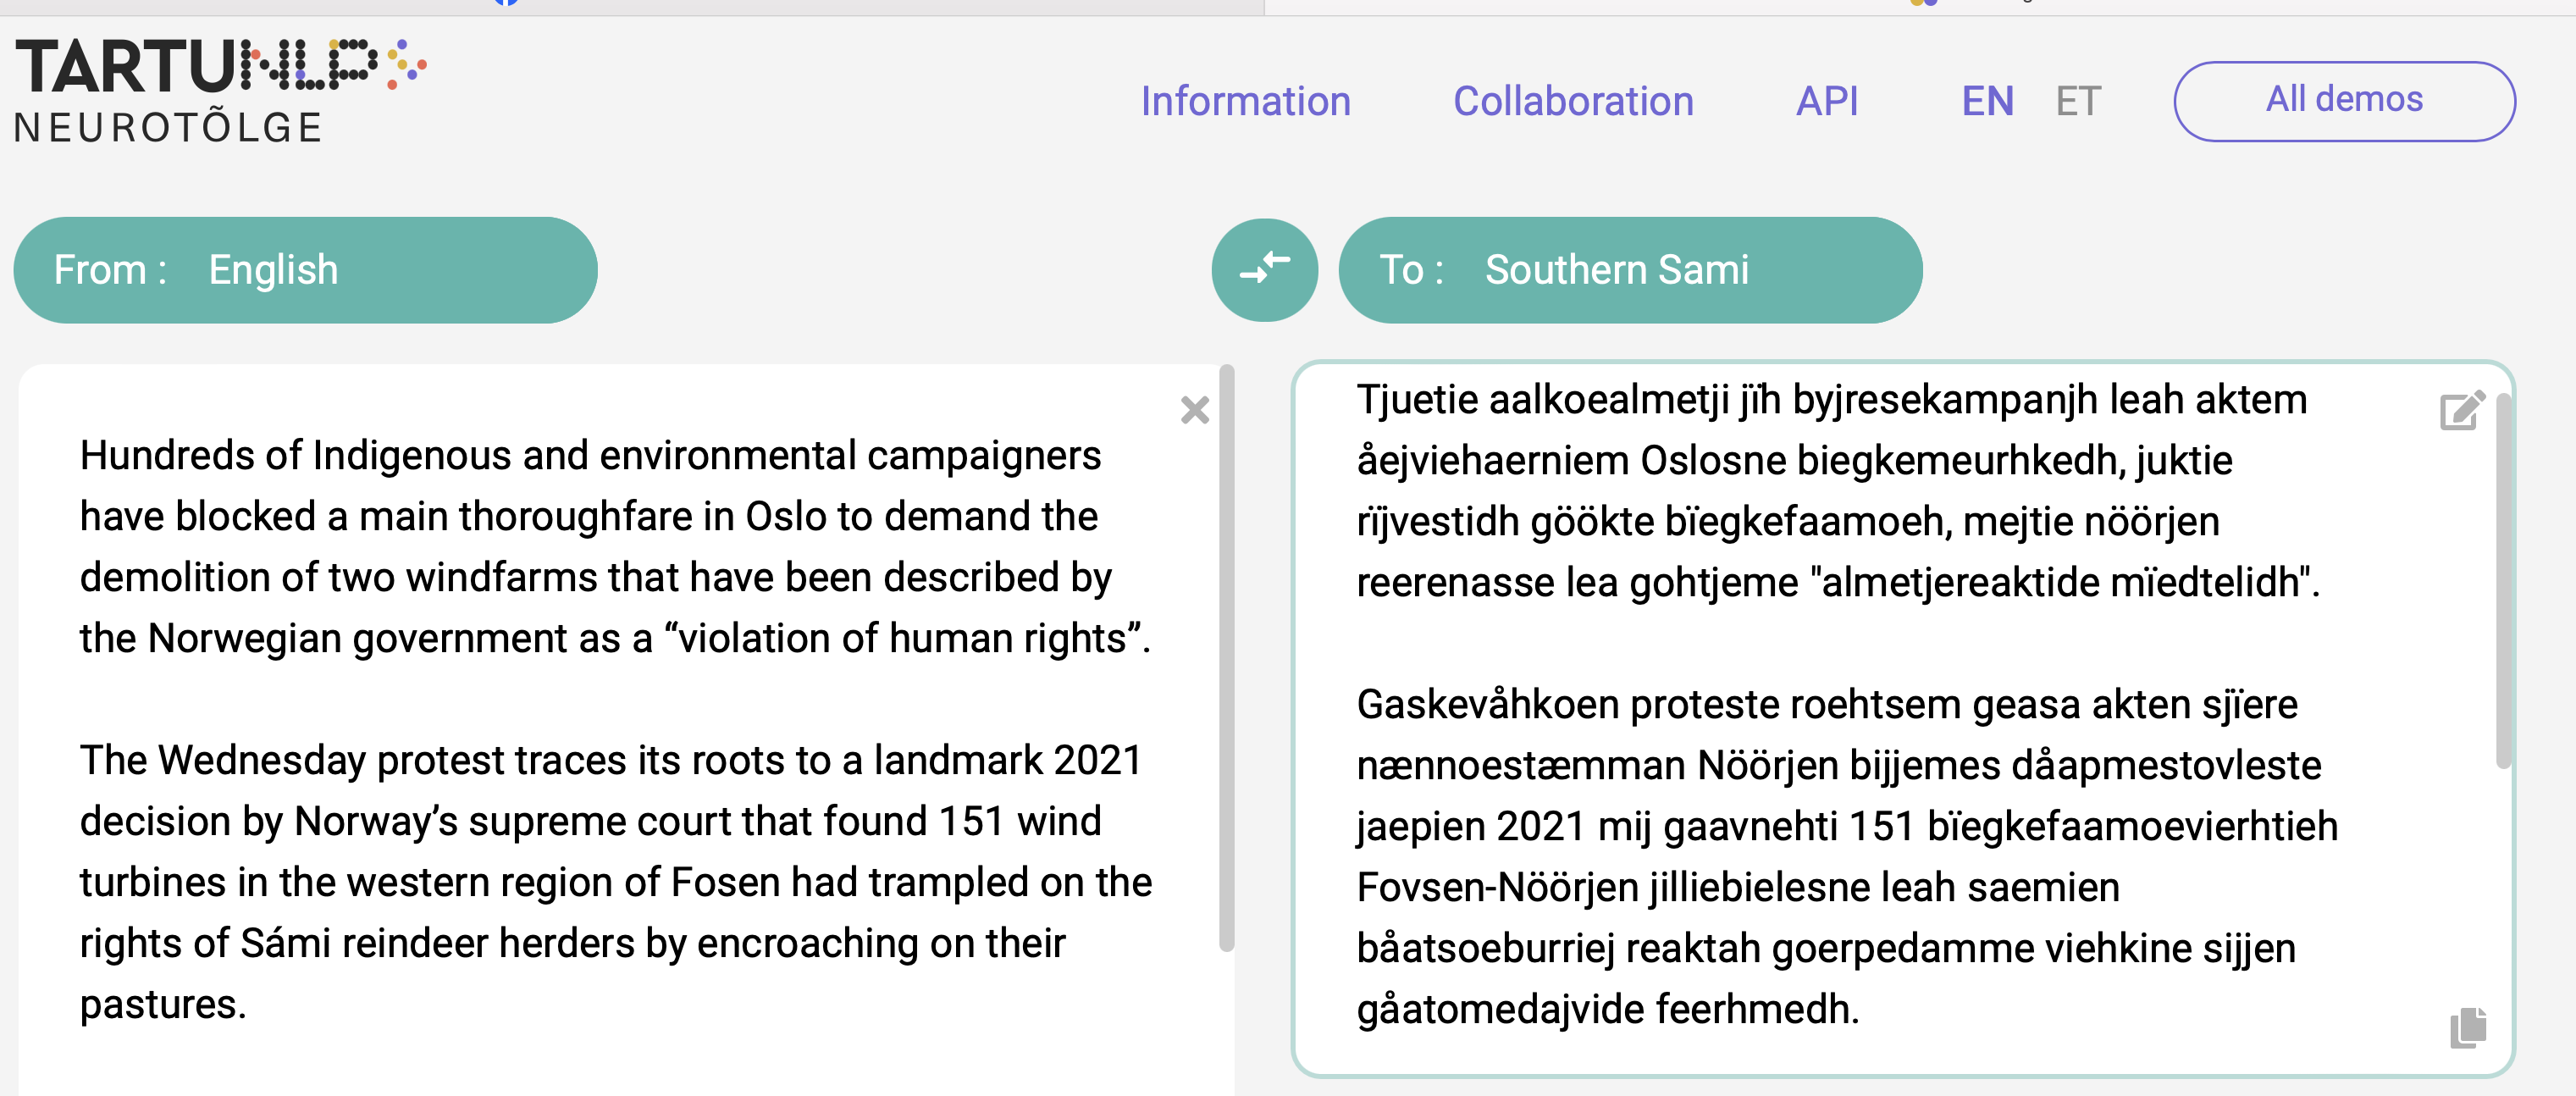
\includegraphics{tartusma.png}}
    \caption{\textit{TARTUNLP Neurotõlge} English-South Sámi MT\label{engsma}}
    \end{center}
    \end{figure*}

Table~\ref{mterr} shows very clearly the immense amount of fails just within the
two first paragraphs of the article.

\begin{table*}[htb]
\begin{center}
\begin{tabularx}{0.8\pagewidth}{lX}
\toprule
\bf Translation fail & \bf Example \\
\midrule
\multicolumn{2}{|c|}{\bf Morpho-syntactical errors} \\
\midrule
Case error (noun) &	\textit{aalkoealmetji} `Indigenous people's'  $>$ \textit{aalkoealmetje} Gen. Pl.$>$Nom. Sg. \\
(pronoun) &	\textit{mejtie} `which' $>$ \textit{mij} Acc. Pl.$>$Nom. Sg.  \\
  &	\textit{reerenasse} `government'$>$\textit{reerenassese} Nom. Sg.$>$Ill. Sg.  \\
   &	\textit{nænnoestæmman} $>$\textit{nænnoestimmeste} Ill.$>$Ela.  \\
    &\textit{protesten} `protest' $>$\textit{proteste} Gen.Sg.$>$Nom.Sg.  \\
Numeral treated as article & \textit{aktem åejviehaerniem}$>$\textit{åejviehaerniem} `one main X'$>$`a main X'\\
& \textit{akten sjïere nænnoestæmman} $>$ \textit{sjïere nænnoestæmman} \\
Active $>$ Passive & \textit{gohtjeme} \textit{gohtjesovveme}\\
Wrong tempus & \textit{feerhmedh} `embrace'  $>$ \textit{feerhmeme}	 Inf$>$Past participle \\
Word order & \textit{rïjvestidh göökte bïegkefaamoeh} $>$ \textit{göökte bïegkefaamoeh rïjvestidh} VO$>$OV\\
\midrule
\multicolumn{2}{|c|}{\bf Lexical issues} \\
\midrule
Wrong word semantics & \textit{byjresekampanjh} `environmental campaigns' $>$  \textit{byjres} `environmental campaigners' \\
& \textit{bïegkefaamoeh} `wind power' $>$ \textit{bïegkefaamoehpark}  `wind power park' \\
& \textit{bïegkefaamoevierhtieh} `wind power ressources' $>$\textit{bïegkefaamoejårrehtsh} `wind power turbines'\\
& \textit{byjresekampanjh} (should be human)  \\
Semantic inadequacy & \textit{gaavnehti} `find out' $>$ \textit{nænnoesti} `decide, implement' \\
Nonsense words & \textit{åejviehaerniem} `main?' $>$ \textit{åejviegæjnoem} `main road' \\
 & \textit{biegkemeurhkedh} $>$ \textit{dahpeme} `close' \\
Literal translation of idiom & `traces its roots' --- \textit{roehtsem geasa} `roots drag' $>$  \textit{vualkove lea} `the origin is' \\
Non-standardized version &	\textit{Oslosne} $>$ \textit{Oslovisnjie} \\
\midrule
\multicolumn{2}{|c|}{\bf Missing parts / Redundancy} \\
\midrule
Missing content word & $>\emptyset$ `to demand' $>$ \textit{krïebpesjidh}\\
Missing logical connector & $>\emptyset$ $>$ \textit{dannasinie} `because' \\
\midrule
\multicolumn{2}{|c|}{\bf Significant meaning changes} \\
\midrule
opposite semantics/value & \textit{feerhmedh} `embrace' (positive) $>$ \textit{gaertjiedamme} (negative) \\
& \textit{viehkine} `with help' (positive) $>\emptyset$  \\
\bottomrule
\end{tabularx}
\end{center}
\caption{\label{mterr} Classification of the errors in English-South Sámi machine translation.}
\end{table*}

The South Sámi text reveals that the content is about campaigns --- Indigenous
people did something in Oslo --- but what did they do? Taking down wind power
--- does that mean the abstract thing? Also, the Norwegian government has called
out others for breaking human rights --- but we know that in reality the
Norwegian government is violating human rights.

The conclusion is that a South Sámi speaker can get a general impression of the
subject area, the involved parties and the place of action, but details of these
actions are unintelligible, and the worst is, the central message is not
conveyed, instead the translation gives the opposite meaning. The Norwegian
government stands out as a helper instead of the culprit.

When the user is proficient in both the source and target languages and is aware
of the potential for such errors, their impact is unlikely to be significant.
However, if the South Sámi output is used uncritically and simply published,
this would have catastrophic consequences and it is unethical.

Additionally, careful reading of neural machine translation output is not an
innate qualification but requires training and strong language intuitions. In a
bilingual society, where typically the majority language has taken over a large
amount of domains and marginalized the domains of the Indigenous languages, even
manual translations can be heavily colored by the majority language.  The
following examples from South Sámi children's literature shows how even highly
qualified translators can choose translations that are literal translations of a
Scandinavian language to the disadvantage of efficient and adequate South Sámi
constructions. `Then Stæjna comes walking with big steps.' is translated with an
adjective and a noun phrase construction (just as in English) as in
ex.~\ref{sma-norsk} whereas South Sámi lexicalizes `with big steps' in a single
adverb \textit{voepsijeslaakan}, cf.\  ex.~\ref{sma-nice}.


\ex.
\ag. Daelie Stæjna båata vaedtsien \textbf{stoerre} \textbf{sïlligujmie}.\label{sma-norsk}\\
then Stæjna come\textsc{.pres.3sg} walking big step\textsc{.pl.com}\\
\bg. Daelie Stæjna \textbf{voepsijeslaakan} båata vaedtsien.\label{sma-nice}\\
then Stæjna with.big.steps\textsc{.adv} come\textsc{.pres.3sg} walking\\



Another children's book's translation uses the inadequate cognate for `door' in
the event of going through a door, and also translates the adpositional
construction in the Scandinavian languages (and English) directly to an
adpositional phrase in South Sámi. However, the meaning of this is not `walking'
but `crashing' through the door.  The South Sámi idiomatic way of saying it uses
the word \textit{okseraejkiem} `door frame' in accusative case as in
ex.~\ref{sma-nice3} rather than \textit{oksen tjïrrh} `door through' as in
ex.~\ref{sma-ugly3}


\exg. Dïhte \textbf{oksen} \textbf{tjïrrh} båata.\label{sma-ugly3}\\
     \textsc{pron.3sg.nom} door\textsc{.gen} through come.crashing\textsc{.3sg}\\
    `She/he/it crashes through the door'

\exg. Dïhte \textbf{okseraejkiem} båata.\label{sma-nice3}\\
    \textsc{pron.3sg.nom} door.frame\textsc{.acc} come\textsc{.3sg}\\
    `She/he/it comes through the door.'

When efficient idiomatic South Sámi constructions are replaced with less elegant
word-by-word translations from the majority language, part of the authentic
South Sámi linguistic structure gets lost.

The work of a human translator is very challenging in the face of bilingualism
because language happens unconsciously. Especially when there is a lack of
external Indigenous language input their own language intuitions get colored by
the majority language.  When neural machine translation suggests syntactic and
idiomatic structures that are heavily derived from majority language input this
can reinforce the tendency towards language shift towards the majority language.

Linguists and language experts, on the other hand, can contextualize, analyze
and see constructions from an analytical standpoint and relate them to other
Uralic languages, giving them a stronger starting point.  Consequently, a
deliberate standardization process informed by a linguistic analysis of the
language's dominant structures holds immense value.

\section{Conclusion}

With the emerging LLM technology a lot of recent research and development on
minority and Indigenous languages is done by outsiders without knowledge of the
languages in question, solely based on data harvested from the net.

In this article, we have illuminated how large language models make implicit
assumptions that do not match the reality of Indigenous languages on various
levels and produce results that can be  problematic, both from an ethical and
linguistic perspective.  We have have shown this in examples from both
corpus-based language generation and machine translation for the endangered
South Sámi language.

As tools for language generation and machine translation are high up on the wish
list of the Indigenous language communities we have worked with, we have
provided an ethical recipe for developers, to ensure a digital future as it is
wanted by the Indigenous language community.  Harvesting corpora in itself is a
time-consuming process involving a trust-based relation between developers and
owners of the language data.  Respecting intellectual property and crediting
authorship is mandatory for both primary and secondary developers.

Language data found in the internet is of varying quality, and developers need
to distinguish between original text and translated text in order to ensure that
the generated language is authentic, and not just, as in our case, ``Norwegian
or Swedish with South Sámi words''.

Considering monolingual users, it is also essential to reduce significant
translation errors that could convey meanings contrary to the original or
disseminate incorrect information.

In practice this means that language experts and community insiders need to be
present to evaluate the output and perform quality assurance.

More clearly, the Indigenous language community itself needs to be part of the
process and make decisions on authentic language and desired output.

Ethical NLP for any language, and for Indigenous languages in particular, must
ask for the needs of the language community and adapt the tools accordingly.

\section*{Ethics Statement}

As an article about ethical ways of working with indigenous language
technologies the article as a whole describes ethics such that it does not need
repeating here, as a summary´:

We discuss the use of Indigenous linguistic data from within the language
community. One of the authors is a member of the South Sámi community, and a
mother tongue speaker.

The method of ethical data management we lay out in this article is aimed at
more sustainable and just management of data. We have implemented it in our own
workflow and development process.

\section*{References$^\star$}\label{sec:reference}

$^\star$ \textit{References in original article use the LREC's awkward
referencing system which has not been reproduced in this post-print author's
version of the article.}

\bibliographystyle{unsrt}
\bibliography{lrec2024}


\end{document}





